\documentclass[fyp]{socreport}
\usepackage[utf8]{inputenc}
\usepackage[english]{babel}
\usepackage{charter}
\usepackage{subcaption}
\usepackage{fullpage}
\usepackage{hyperref}
\usepackage{amsmath}
\usepackage{booktabs}
\usepackage{graphicx}
\usepackage{forest}
\usepackage[backend=biber,
style=ieee,
doi=false,
url=true,
sorting=none]{biblatex}
\newcommand{\fixme}[1]{#1}
\newcommand{\DRAFT}{
\begin{center}
\textbf{DRAFT! --- \today\ --- DRAFT!}
\end{center}}


\addbibresource{socreport.bib}

\begin{document}
\pagenumbering{roman}
\projyear{2019/20}
\projnumber{H226080}
\author{Kuan Sheng Yuan, Jethro}
\title{Event-Driven Visual-Tactile Learning for Robots}
\advisor{Dr.\ Harold Soh}
\deliverables{
  \item Report: 1 Volume}
\maketitle

\begin{abstract}
  \DRAFT
  In this work, we contribute an event-driven visual-tactile perception system,
  built on spiking neural networks. Our perception system is trained, and tested
  end-to-end on novel multi-modal event-based data for two sensor modalities:
  (1) Tactile data, from our biologically-inspired fingertip tactile sensor,
  NeuTouch and (2) visual data, from the Prophesee camera. We evaluate our
  system on two robotic tasks: container classification, and slip detection. On
  both tasks, we observe good classification accuracies relative to standard
  deep learning methods. Our system can be run on neuromorphic hardware, making
  this a crucial first step towards enabling power-efficient, intelligent
  robots.

  \begin{keywords}
    Spiking Neural Networks, Multi-modal Machine Learning
  \end{keywords}

  \begin{implement} Python 3, PyTorch
  \end{implement}
\end{abstract}

\listoffigures
\listoftables
\tableofcontents

\chapter{Introduction\label{cha:intro}}

Human beings are blessed with innate abilities to integrate sensory information
from different stimuli. Our sense of smell, hearing, touch, vision, and taste
each contribute to how we perceive and act in the world. Consider the scenario
of fetching a carton of soy-milk from the fridge; humans use vision to locate
the carton, and are also able to infer from grasping the object, the amount of
soy-milk the carton contains. These actions (and inferences) are performed
robustly using a power-efficient neural substrate --- compared to popular deep
learning approaches for using multiple sensor modalities in artificial systems,
human brains require far less energy~\cite{li2016energyefficiency}.

In this work, we take crucial steps towards efficient visual-tactile perception
for robotic systems. We gain inspiration from biological systems, which are
\emph{asynchronous} and \emph{event-driven}. In contrast to resource-hungry deep
learning methods, event-driven perception offers an alternative approach that
promises power-efficiency and low-latency --- features that are ideal for
real-time mobile robots. However, event-driven systems remain under-developed
relative to standard synchronous perception methods~\cite{pfeiffer2018deep}.

We make multiple contributions that advance event-driven visual-tactile
perception. First, to enable richer tactile sensing, we use the NeuTouch
fingertip sensor. Compared to existing commercially-available tactile sensors,
NeuTouch's neuromorphic design enables scaling to larger number of taxels while
retaining low latencies.

Next, we investigate multi-modal (visual-tactile) learning using the NeuTouch
and the Prophesee event-based camera. Specifically, we develop a
\emph{visual-tactile spiking neural network} (VT-SNN) that incorporates both
sensory modalities for supervised-learning tasks. Different from conventional
deep artificial neural network (ANN) models, SNNs process discrete spikes
asynchronously, and thus, are arguably better suited to the event data generated
by our neuromorphic sensors. In addition, SNNs can be used on efficient
low-power neuromorphic chips such as the Intel Loihi~\cite{davies2018loihi}.

Our experiments center on two robot tasks: object classification and
(rotational) slip detection. In the former, we tasked the robot to determine the
type of container being handled and amount of liquid held within. The containers
were opaque with differing stiffness, and hence, both visual and tactile sensing
are relevant for accurate classification. We show that relatively small
differences in weight ($\approx 30$g across 20 object-weight classes) can be
distinguished by our prototype sensors and spiking models. Likewise, the slip
detection experiment indicates rotational slip can be accurately detected within
$0.08$s (visual-tactile spikes processed every $\approx 1$ms). In both
experiments, SNNs achieved competitive (and sometimes superior) performance
relative to ANNs with similar architecture.

The work presents an exciting opportunity to enable power-efficient intelligent
robots. Presented with labeled data, an event-driven perception network can be
trained end-to-end, and used on neuromorphic chips as robotic controllers.

\section{Research Outline}

In \autoref{cha:background}, we first provide a comprehensive study on SNNs. We
discuss why and when we should use spiking neural networks, and how to train
them. Crucially, we draw similarities between spiking neural networks and
recurrent neural networks, a recently discovered property that enables the
end-to-end training of these networks using gradient-based methods.

In \autoref{cha:vtsnn}, we contribute an event-driven visual-tactile
spiking-neural network (VT-SNN), which enables fast perception on two
event-based sensors: the NeuTouch~\cite{aiskinLee}, and the Prophesee event
camera. Here, we detail the experimental setups for the robotic tasks: object
classification and slippage detection. We discuss our experimental results, and
demonstrate that spiking neural networks achieve competitive (and sometimes
superior) performance over deep learning methods, and in addition having the
unique property of early classification.

This thesis was originally an exploratory project on spiking neural networks.
In the duration of this research, several different research directions have
been explored. In the chapters that follow, we discuss research directions we
have taken that were later abandoned.

In \autoref{cha:snnrl}, we evaluate the feasibility of spiking neural networks
as agents in a reinforcement learning setting. Reinforcement learning
environments are often temporal in nature, due to the interdependence between
states and actions in the environment. We hypothesised that spiking neural
agents were well suited in many reinforcement learning settings.

\section{Individual Contributions}
The event-driven visual-tactile perception system is a joint work between our
group, the Collaborative Learning \& Adaptive Robots (CLeAR) group, and the TEE
research group.

The TEE research group contributed the novel NeuTouch tactile sensor, which was
used to collect data for the tactile modality. The CLeAR group contributed: (1) a
visual-tactile spiking neural network (VT-SNN) that leverages multiple event
sensor modalities, (2) systematic experiments demonstrating the effectiveness of
our event-driven perception system on object classification and slip detection,
with comparisons to conventional ANN methods, and (3) visual-tactile event
sensor datasets comprising more than 50 different object classes across the
experiments, including RGB images and proprioceptive data from the robot.

Among the contributions of the CLeAR group, my individual contributions include
the experimentation (training and evaluation) of the VT-SNN models, as well as
some guidance on the ANN models. I am also looking into running these models on
neuromorphic hardware, to quantify the performance and power gains of using the
spiking models. During the research process, I also maintained the code
repository at high-quality. Model training was designed to be reproducible, and
parameter searches could be done efficiently across multiple GPUs. Different
experimental runs could also be plotted, and their results aggregated for later
analyses.

All work in subsequent chapters ()\fixme{fill this in}
are my own.

\chapter{Background\label{cha:background}}

This chapter provides background knowledge about spiking neural networks. It
reviews the differences between deep neural networks, and spiking neural
networks (\ref{sec:gener-neur-netw}). It introduces the basics of spiking neural
networks (\ref{sec:spiking-neuron-model}), and its benefits
(\ref{sec:motiv-spik-neur}). Finally, we discuss how to train spiking neural
networks (\ref{sec:train-spik-neur}), and give a short conclusion with future
directions.

\section{The Generations of Neural Networks\label{sec:gener-neur-netw}}

Neural network models can be classified into three generations, according to
their computational units: perceptrons, non-linear units, and spiking
neurons~\cite{MAASS19971659}. Perceptrons can be composed to produce a variety
of models, including Boltzmann machines and Hopfield networks. One
characteristic feature of perceptrons is that only give digital output.

Non-linear units apply an activation function with a continuous set of possible
output values to a weighted sum of the inputs. Classic examples of networks of
this second generation include feed-forward and recurrent sigmoidal neural
networks. These networks are able to compute functions with analog input and
output. Non-linear units are currently the most widely used computational unit,
and is responsible for the explosion of progress in machine learning research,
in particular, the success of deep learning. This is largely because networks
built with these units are trainable with well-researched gradient-based
methods, such as backpropagation.

Despite being biologically inspired, second-generation neural networks (ANNs)
bear little resemblance to the human cortex. In contrast to the digital
computation in ANNs, networks of neurons perform fast analog computations. This
inspired a the third generation of neural networks use computational units
called \emph{spiking neurons}, which communicate via discrete spikes. Much like
our biological neurons, spiking neurons are connected to each other at synapses,
receiving incoming signals at the dendrites, and sending spikes to other
downstream neurons via the axon. Each computational unit stores its membrane
potential, which fluctuates over time based on well-defined neuronal dynamics.
Rather than firing at each propagation cycle, these computational units fire
only when their individual membrane potentials crosses its firing threshold.

\begin{table}
  \centering
  \small
  \begin{tabular}{ l|ccc }
    \hline
    \hline
    \textbf{Name} & \textbf{Input} & \textbf{Output} & \textbf{Examples} \\
    \hline
    (1) Perceptrons & Digital & Digital & Hopfield Networks, Boltzmann Machines \\
    (2) Non-linear Units & Digital/Analog & Digital/Analog & Feed-forward \& Recurrent ANNs \\
    (3) Spiking Neurons & Analog & Analog & Feed-forward SNNs \\
    \hline
    \hline
  \end{tabular}
  \normalsize
  \caption{\label{tab:nn_generations} The three generations of neural networks. }
\end{table}

Henceforth, we shall term second-generation neural networks artificial neural
networks (ANNs), and third-generation neural networks spiking neural networks
(SNNs).

\section{Motivating Spiking Neural Networks\label{sec:motiv-spik-neur}}

Since ANNs have excellent performance, and can handle both digital and analog
input and output, why should we bother with spiking neural networks? In this
section, we motivate spiking neural networks from various perspectives.

\subsection{Information Encoding via Spikes}

To directly compare ANNs and SNNs, one can consider the real-valued outputs of
ANNs to be the firing rate of a spiking neuron in steady state. In fact, this
scheme, termed \emph{rate coding}, has been used to explain computational
processes in the brain~\cite{pfeiffer2018deep}.

However, experiments have shown that different actions are taken based on single
spikes~\cite{stemmler96_singl_spike_suffic}. In addition, the humans are capable
of performing tasks such as visual pattern analysis and pattern classification
in 100ms~\cite{thorpe2001spike}. Rate coding strategies are far too inefficient
for the rapid information transmission required for sensory processing. In
addition, the firing distribution of biological neurons is heavily skewed
towards lower firing rates. To obtain a good estimate of the firing rate, many
spikes would be required.

Different from ANNs, spiking neuron models are able to encode information beyond
the average firing rate: these models also utilize the relative timing between
spikes~\cite{guetig14_to_spike_or_when_to_spike}, or spike phases (in-phase or
out-of-phase). These time-dependent codes are termed \emph{temporal codes}, and
play an important role in biology. It has also been successfully demonstrated
that temporal coding achieves competitive empirical performance on
classification tasks for both generated datasets, as well as image datasets like
MNIST and CIFAR~\cite{comsa19_tempor_codin_spikin_neural_networ}.

There is additional benefit to encoding information directly in the temporal
domain. Architectures for atemporal artificial neural networks that use a memory
mechanism, such as the LSTM~\cite{hochreiter1997long}, require every neuron wait
on the activation of all neurons in previous layers before producing an answer.
In spiking neural networks, the output layers spike over time, and predictions
can be made at any time-step. Hence, SNNs are able to operate in two regimes.
The first regime is a highly accurate but slow regime, where predictions are
made at later time-steps. This is the regime that atemporal ANNs support, where
predictions are typically made only after a fixed time-step. The second regime
is a low accuracy but fast regime, where the network fast predictions, at a much
lower accuracy. This behaviour mirrors the speed-accuracy tradeoff observed in
human decision-making~\cite{comsa19_tempor_codin_spikin_neural_networ}, and we
also observe and exploit this property in our work described
in~\autoref{cha:vtsnn}.

By observing that biological neurons use spikes to communicate information, a
wide range of coding schemes have been developed. Each of these codes have
different information capacities, and their pros and cons. We defer this
discussion to~\cite{thorpe2001spike}, but summarize the coding schemes
in~\autoref{tab:coding_schemes}. Spiking neural networks are able to take
advantage of these various coding schemes.

\begin{table}
  \centering
  \small
  \begin{tabular}{l|c}
    \hline
    \hline
    \textbf{Coding Scheme} & \textbf{Encoding of Information} \\
    Rate Coding & Firing rate of neurons \\
    Count Code & Count of number of neurons that spike during in time window \\
    Binary Code & Binary pattern of length $N$ from $N$ neurons (e.g. $0010$,
                  where the third neuron spiked) \\
    Temporal Code & Time of each spike in the spike
                    train \\
    Rank Code & Order in which neurons fire \\
    Synchrony Code & Patterns from a population of neurons \\
    \hline
    \hline
  \end{tabular}
  \normalsize
  \caption{Coding Schemes in Spiking Neural Networks}
  \label{tab:coding_schemes}
\end{table}

\subsection{Practical Benefits}

The ability to communicate information in a small number of spikes has immense
practical benefits.

\subsubsection{Real-time Performance and Parallelism}

The analog communication modeled in spiking neurons allow for naturally parallel
and high-speed computation. The promise of real-time performance is a key
motivator behind the development of neuromorphic hardware. Typical hardware such
as the everyday computer uses the von Neumann architecture, which separates
memory and processing, which has severe implications on performance.
Neuromorphic hardware collocates memory and processing, overcoming the von
Neumann bottleneck~\cite{Backus_1978}.

\subsubsection{Power Efficiency}
Next, the primary motivation cited in present-day literature is the
power-efficiency of spiking neural networks. First, less energy is used in
propagating fewer spikes. Second, communication via spikes is much more
computationally efficient than the floating point arithmetic performed in
artificial neural networks. This low energy footprint is a highly desirable
trait in robotics applications.

\subsubsection{Online Learning and Fault Tolerance}

Biological neurons brain evolve and adapt as time passes, creating new
connections, and destroying old ones. While the phenomenon of
\emph{neuroplasticity} is not yet well understood, it is hoped that the learning
mechanisms behind human intelligence will inspire a new generation of online
learning algorithms.

Neurons also frequently perish, and the human brain has the ability to
self-heal. In the same way, spiking neural network architectures can be designed
to possess the same self-healing and fault tolerance characteristics. This is a
desirable trait for systems where uptime is critical.

\subsection{Biological Plausibility\label{bioplausible}}
In addition to having practical benefits, spiking neural networks more closely
model the biological brain. A faction of the machine learning and neurobiology
community strives for emulation of the biological brain. There are several
incompatibilities between ANNs and the current state of neurobiology that are
difficult to reconcile.

First, neurons in ANNs communicate via continuous-valued activations. In
contrast, it is well established that biological neurons communicate by
broadcasting spike trains --- trains of action potentials --- to downstream
neurons. The spikes are to a first-order approximation of uniform amplitude,
unlike the continuous-valued activations of ANNs.

Second, backpropagation as a learning procedure also presents incompatibilities
with the biological brain~\cite{TAVANAEI201947}, explained in further detail
in~\autoref{sec:diff-train}. This result motivates the search for alternative
learning mechanisms for spiking neural networks.

\subsection{Summary}
In conclusion, the main motivations for spiking neural networks are the
following:

\begin{itemize}
  \item Neuromorphic hardware can overcome the von Neumann bottleneck
  \item When combined with neuromorphic hardware, SNNs can:
  \begin{itemize}
    \item achieve real-time performance via asynchronous spiking communication
    \item achieve low power consumption from sparse spiking computation
    \item implement plasticity-inspired online learning mechanisms
    \item Fault tolerance beyond what von Neumann architectures can provide
  \end{itemize}
  \item Some SNNs have biologically-plausible neuron models, which can help
  answer open questions in neuroscience
\end{itemize}

\section{Neuron Models\label{sec:spiking-neuron-model}}

Neuron models are mathematical models that describe the underlying neuron
dynamics: how electrical signals propagate from inputs to outputs, and the
changes in the neurons internal state, such as the membrane potential.

Many of these neuron models are modeled after the biological neuron, which has a
few main components:

\begin{description}
  \item[{Dendrites}] Neurons receive input signals at the dendrites, which
    transmit incoming electrical signals to the cell body.
  \item[{Cell Body}] The cell body is responsible for ``processing'' the input
    from the dendrites. The typical behaviour is to accumulate the electrical
    input from the dendrites. Once the cell's membrane potential crosses a
    certain threshold, it spikes, and sends an output signal through the axon.
  \item[{Axons}] The axon receives electrical signals from the cell body.
    Electrical signals propagate down to axon terminals, which control the
    release of neurotransmitters.
\end{description}

The perceptron was biologically-inspired, and has an analogous representation
that may be helpful for understanding, which we present
in~\autoref{fig:bio_neuron}.

\begin{figure}[ht]
  \begin{subfigure}{.5\textwidth}
    \centering
    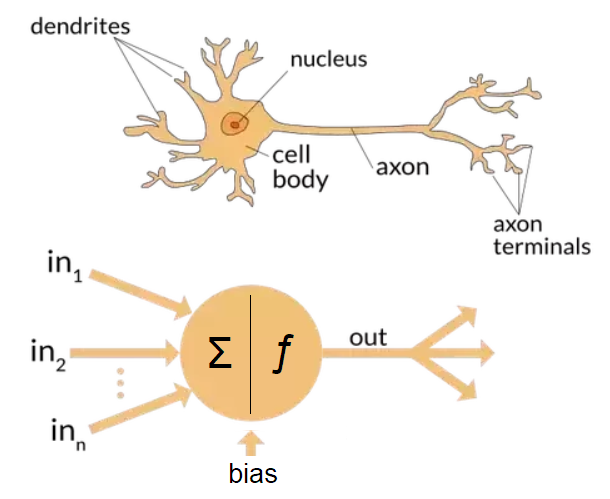
\includegraphics[width=0.8\textwidth]{images/biological_neuron_perceptron.png}
  \end{subfigure}
  \begin{subfigure}{.5\textwidth}
    \centering
    \begin{tabular}{|l|l|}
      \hline
      \hline
      \textbf{Biological Neuron} & \textbf{Perceptron} \\
      \hline
      Dendrites & Inputs \\
      Cell Body & Processing input: $f(\sum \textbf{w} \cdot \textbf{i})$ \\
      Axon (Terminals) & Output \\
      \hline
      \hline
    \end{tabular}
  \end{subfigure}
  \caption{The biological neuron~\cite{tds_artif_biolog_neural_networ}, in contrast with a perceptron.}
  \label{fig:bio_neuron}
\end{figure}

In this section, we present a taxonomy of neuron models. These neuron models
vary in computational and implementation complexity. We discuss some of them in
brief, and conduct a thorough review of the Spike Response Model (SRM). For a
more in-depth treatment of spiking neuron models, we refer you to~\cite{izhikevich2004model}.

\begin{figure}[t]
    \centering
    \begin{forest}
      for tree={align=left}
      [\textbf{Neuron Models}
      [\textbf{McCulloch-Pitts}]
       [\textbf{Spiking Neurons}
       [{\textbf{Biologically-plausible} \\
         - \small{Hodgkin-Huxley~\cite{hodgkin1952quantitative}} \\
         - \small{Morris-Lecar\cite{morris81_voltag_oscil_barnac_giant_muscl_fiber}}}]
       [\textbf{Biologically-inspired}
       [\textbf{Simplifications} \\
       - \small{FitzHugh-Nagumo~\cite{fitzhugh1955mathematical}} \\
       - \small{Izhikevich~\cite{izhikevich2003simple}}]
       [\textbf{Integrate-and-Fire (IF)} \\
       - \small{IF~\cite{abbott99_lapic_introd_integ_and_fire}} \\
       - \small{(Fractional) Leaky IF~\cite{teka14_neuron_spike_timin_adapt_descr}} \\
       - \small{Spike-response~\cite{gerstner2001framework}}
       ]]]
      ]
    \end{forest}
    \caption{A taxonomy of popular spiking neuron models.}
    \label{fig:snm_taxonomy}
  \end{figure}

\subsection{McCulloch-Pitts}
Activation functions such as the sigmoid function, and hyperbolic tangent
function can be implemented at the hardware level in the McCulloch-Pitts neuron
model. However, these models use digital input and output, which means they have
a higher footprint than spiking neuron models which perform analog computation.

\subsection{Biologically-plausible Models}
The Hodgkin-Huxley~\cite{hodgkin1952quantitative} model is a mathematical model
that uses four-dimensional non-linear differential equations to model the neuron
dynamics, using the transfer of ions as the medium. This model is popular among
the neuroscientific community, for accurately modelling the biological process.
The Morris-Lecar~\cite{morris81_voltag_oscil_barnac_giant_muscl_fiber} model is
a simplification of the Hodgkin-Huxley model, which is more easily implementable
in hardware.

\subsection{Biologically-inspired Models}
Some biologically-inspired models often sacrifice biological-plausibility for
ease of implementation. These models have a smaller number of parameters,
resulting in models that are not only easier to train, but also have a smaller
energy footprint. These models include the
FitzHugh-Nagumo~\cite{fitzhugh1955mathematical}, and the
Izhikevich~\cite{izhikevich2003simple} model.

A particularly notable family of biologically-inspired models in the
integrate-and-fire family. These models maintain as state, the membrane
potential of the neuron, accumulating charge from input neurons. The leaky
integrate-and-fire model introduces an additional ``leak'' term, which controls
the decay of the neuron's membrane potential over time.

\section{The Spike-response Model}

The spike-response model~\cite{gerstner2001framework} is a generalization of the
leaky integrate-and-fire model. We review this model because this neuron model
is used in SLAYER~\cite{NIPS2018_7415}, the framework we use in our experiments.

Rather than modelling the neuronal dynamics using differential equations, the
SRM model uses convolutional filters, a property that makes the simulation and
training of these spiking models easy. In contrast to the leaky IF model, the
refractory behaviour of the neuron is also captured, which has allowed it to
better fit spiking data~\cite{jolivet04_gener_integ_and_fire_model}.

In this model, a neuron is characterized by a single variable $\mu$, the
membrane potential of the cell. Suppose that the neuron has fired its last spike
at time $\hat{t}$. Then, in the most general formulation, at each time
$t > \hat{t}$, the state of the cell is expressed as an integral over the
previous timesteps:

\begin{equation}
  \label{eq:srm}
  \mu(t) = \eta(t - \hat{t}) + \int_{-\infty}^{+\infty}\kappa(t - \hat{t}, s)I(t - s) ds
\end{equation}

where $\eta$ describes the form of the action potential, $\kappa$ is the linear
response to an input pulse, and $I(t)$ is the stimulating current. In most
spiking neural network architectures, the imposed current $I(t)$ is instead
described as a weighted sum of presynaptic inputs, and the equation can be
rewritten as:

\begin{equation}
  \label{eq:srm}
  \mu(t) = \eta(t - \hat{t}) + \sum_{j} \sum_{f} w_{j}\epsilon(t - \hat{t}, t-t_{j}^{f})
\end{equation}


where $\epsilon$, the spike response kernel, is obtained by convolving the
kernel $\kappa$ with the time course of the presynaptic input.

A common form for the refractory kernel $\eta$ is:

\begin{equation}
  \label{eq:srm_eta}
  \eta(t) = - \eta_{0} \textrm{exp} \left(- \frac{t}{\tau}\right) \mathcal{H}(t)
\end{equation}

where $\eta_{0}$ is the amplitude of the relative refractorines, $\tau$ is a
decay time constant, and $\mathcal{H}$ is the Heaviside step function.

SLAYER uses the SRM model, and formulates it this way. Suppose that the neuron
receives an input spike train,
$s_i(t) = \sum_{f} \delta\left( t - t_i^{(f)} \right)$. The spike train is
represented as a sum of Dirac delta functions with \(\delta(x) = 0\) for
\(x \ne 0\) and \(\int_{-\infty}^{\infty} \delta(x)dx = 1\). In the spike
response model, incoming spikes are converted into a \emph{spike response
  signal}, $a_{i}(t)$, by convolving $s_{i}(t)$ with a spike response kernel
$\epsilon(\cdot)$: $a_{i}(t) = (\epsilon \ast s_{i})(t)$. The refractory
response of the neuron can also be represented with a refractory kernel
$\eta(\cdot)$, giving the formula for the refractory response:
$(\eta \ast s)(t)$ for the neuron's spike train $s(t)$.

Each spike response signal is scaled by a synaptic weight $w_{i}$, to generate a
post synaptic potential (PSP). The neuron's state is then given by the equation:

\begin{equation}
  \label{eq:slayer_srm}
  \mu(t) = (\eta \ast s)(t) + \sum_{i} w_{i}(\epsilon \ast s_{i})(t) = (\eta \ast s)(t) + \boldsymbol{w}^{T} \boldsymbol{a}(t)
\end{equation}

The neuron produces an output spike when membrane threshold $\theta$ is
reached. The spike function $f_{s}(\cdot)$ is defined as:

\begin{equation}
  \label{eq:slayer_spike_fn}
  f_{s}(\mu) : \mu \rightarrow s, s(t) := s(t) + \delta(t - t^{f+1}) \text{
    where } t^{f+1} = \textrm{min}\left\{t: \mu(t) = \theta, t > t^{f}\right\}
\end{equation}

\section{Neuromorphic Hardware\label{neuromorphic}}

To obtain the full benefits of spiking neural networks, they need to be deployed
on specialized neuromorphic hardware. In a traditional Von Neumann architecture,
the logic core operates on data fetched sequentially from memory. In
neuromorphic chips, both computation and memory are instead distributed across
computational units that are connected via synapses. Henc, the neuronal
architecture and parameters play a key role in information representation and
define the computations that are performed.

It has also been observed that spike-trains in the mammalian brain are often
sparse in time, suggesting that timing and relative timings of spikes encode
large amounts of information. Neuromorphic chips implement this same sparse,
low-precision communication protocol between neurons on the chip, and by
offering the same asynchronous, event-based parallelism paradigm that the brain
uses, are able to perform certain workloads with much less power than Von
Neumann chips.

Examples of such chips include IBM's TrueNorth~\cite{Merolla668} and Intel's
Loihi~\cite{davies2018loihi}. Loihi features 128 neuromorphic cores, each of
which implementing 1024 spiking neural units. The mesh protocol further supports
scaling up to 4096 on-chip cores. The large number of computational units and
their interconnectivity is a common feature in neuromorphic chips.

~\citeauthor{blouw18_bench_keywor_spott_effic_neurom_hardw} quantified the
trade-offs between network size, inference speed, and energy cost between
different hardware. The comparison showed that the Intel Loihi was 100 times
more efficient than a GPU, with inference speeds also being three times
faster~\cite{blouw18_bench_keywor_spott_effic_neurom_hardw}.

Because spiking neural networks have not yet been successfully trained on many
tasks, neuromorphic chips has seen little practical use. These chips have only
recently been successfully used in robotic navigation~\cite{SnnSlam}, and
solving graph problems by manual construction of the network
graph~\cite{Severa2016SpikingNA}.

\section{Training Spiking Neural Networks\label{sec:train-spik-neur}}

It is desirable to train spiking neural networks to perform arbitrary tasks,
utilizing power-efficient neuromorphic chips that break the Von Neumann
bottleneck. However, spiking neural networks have yet to achieve superior
performance relative to their ANN counterparts. In this section, we first
discuss the difficulties in training SNNs. Then, we provide a taxonomy of
training strategies.

\subsubsection{Difficulties in Training\label{sec:diff-train}}

Because backpropagation has been effective in training artificial neural
networks, the natural approach is to attempt to apply it to spiking neural
networks. However, consider the chain rule in backpropagation:

\begin{equation}
  \label{chainrule}
  \delta_{j}^{\mu}=g^{\prime}\left(a_{j}^{\mu}\right) \sum_{k} w_{k j} \delta_{k}^{\mu}
\end{equation}

\(\delta_{j}^{\mu}\) and \(\delta_{k}^{\mu}\) denote the partial derivatives of
the cost function for input pattern \(\mu\) with respect to the net input to
some arbitrary unit \(j\) or \(k\). Unit \(j\) projects feed-forward connections
to the set of units indexed by \(k\). \(g(\cdot)\) is the activation function
applied to the net input of unit \(j\), denoted \(a_j^{\mu}\), \(w_{kj}\) are
the feedforward weights projecting from unit \(j\) to the set of units indexed
by \(k\).

The chain rule formulation presents two key challenges. First, the gradients
\(g'(\cdot)\) requires derivatives, but \(g(\cdot)\) in spiking neurons is
represented by sum of Dirac delta functions, for which derivatives do not exist.
The non-differentiability.

Second, the expression \(\sum_{k} w_{k j} \delta_{k}^{\mu}\) uses feedforward
weights in a feedback fashion. This mean that backpropagation is only possible
in the presence of symmetric feedback weights, but these do not exist in the
brain. This is also known as the ``weight-transport''
problem~\cite{grossberg1987competitive}. A more practical problem the usage of
non-local information during error assignment. This makes the backpropagation
incompatible with many neuromorphic hardware implementations, such as the Loihi:
the learning rules of the Loihi are constrained to be of a sum-of-products form.

In the following sections, we present training methods that work around these
difficulties, according to the following classification:

\begin{description}
  \item[Usage of Gradients] Recent advancements in the field have opened up the possibilities of using gradient-based methods for training spiking neural networks. We classify the learning algorithms based on whether they utilize gradient information for learning.
  \item[Offline/Online] Since many neuromorphic hardware implementations impose strict restrictions on the neuron update rules, many learning algorithms use simulations on Von Neumann hardware to learn the SNN weights before deploying them on hardware. We classify the learning algorithms based on whether online learning on neuromorphic chips is possible.
\end{description}

\begin{table}[ht]
  \centering
  \begin{tabular}{|l|l|l|}
    \hline
    & \textbf{Non-gradient based} & \textbf{Gradient-based} \\
    \hline
    \textbf{Offline-only} & \begin{tabular}{@{}l@{}}
                        \small
                        Evolutionary Algorithms
                      \end{tabular} & \begin{tabular}{@{}l@{}}
                                        \small
                                        ANN $\rightarrow$ SNN \\
                                        Smooth models \\
                                        Surrogate Gradients
                                      \end{tabular}\\
    \hline
    \textbf{Online} & \begin{tabular}{@{}l@{}}
                        \small
                        Local Learning Rules
                      \end{tabular} & \begin{tabular}{@{}l@{}}
                                        \small
                                        Surrogate Gradients + Random BP
                                      \end{tabular}\\
    \hline
  \end{tabular}
  \caption{A taxonomy of learning algorithms for spiking neuron models.}
  \label{tab:snm_train_taxonomy}
\end{table}

\subsubsection{Local Learning Rules}

Local learning rules are simple fixed rules, that tells a neuron how to update
its weights for each training example. These rules often only use information
from neighbouring neurons, and can be easily implemented on neuromorphic
hardware. The earliest of such rules is Hebbian
learning~\cite{hebb1949organization}, which can be summarized as ``neurons which
fire together wire together''.

A recent, and much more popular learning rule is the spike-timing-dependent
plasticity rule (STDP). Central to these learning rules is the theme that neuron
spike ordering and their relative timings encode information. STDP adjusts the
strength of connections between neurons using the relative timing of a neuron's
output and its input potentials.

In machine learning terminology, the weights of the synapses are adjusted
according to fixed rules for each training example. Each synapse is given a
weight \(0 \le w \le w_{\max}\), characterizing its strength, and its change
depends on the exact moments \(t_{pre}\) of pre-synaptic spikes and \(t_{post}\)
of post-synaptic spikes~\cite{sboev18_spikin_neural_networ_reinf_learn}:

\begin{equation}
  \Delta w=\left\{\begin{array}{l}{
                    -\alpha \lambda \cdot \exp \left(-\frac{t_{\mathrm{pre}}-t_{\mathrm{post}}}{\tau_{-}}\right),
                    \text {if } t_{\mathrm{pre}}-t_{\mathrm{post}}>0} \\
                    {\lambda \cdot \exp \left(-\frac{t_{\mathrm{post}}-t_{\mathrm{pre}}}{\tau_{+}}\right),
                    \text {if } t_{\mathrm{pre}}-t_{\mathrm{post}}<0}
                  \end{array}\right.
\end{equation}

where \(\tau_{+}\) and \(\tau_{-}\) are time constants. \(\tau_{+} = 16.8ms\)
and \(\tau_{-} = 33.7ms\) are reasonable approximations obtained experimentally.

Because the rules are local, these local learning rules fall within the
unsupervised learning paradigm of machine learning. However, more recently,
variants of STDP such as reward-modulated
STDP~\cite{legenstein08_learn_theor_rewar_modul_spike} have been proposed to
allow for neurons to learn to update synaptic weights to maximize the global
reward of a system.

Libraries such as BindsNET~\cite{10.3389/fninf.2018.00089} that simulate SNNs on
Von Neumann computers implementing these rules. Recent attempts have been made
to combine Reinforcement Learning and STDP:\@ both in solving reinforcement
learning problems~\cite{10.3389/fninf.2018.00089}, and using the reinforcement
learning framework to train
SNN~\cite{10.3389/fnbot.2019.00018,10.3389/fnins.2018.00435}. However, SNNs
trained using the STDP learning rule have yet to achieve comparable performance
compared to ANNs on relatively simple datasets like MNIST~\cite{TAVANAEI201947}.

\subsubsection{Evolutionary Algorithms}

In the absence of gradients, neuroevolution is a popular option. Evolutionary
algorithms were once thought to be ineffective for training neural networks,
which have large parameter spaces. However, advancements in the algorithmic
front have made them feasible for solving challenging reinforcement learning
problems~\cite{such17_deep_neuroev}.

One such evolutionary algorithm that can be easily applied to spiking neural
networks is differential evolution (DE). In differential evolution, a population
of candidate solutions are maintained. At each timestep, the parameters of these
agents are tweaked, and the candidates is evaluated. In some variants of DE, a
reproduction step involving crossing-over of weights between candidate solutions
is also introduced. The agent that has the best performance is returned after
some stopping criterion (e.g. time-step) is reached. Evolutionary algorithms
tend to be computationally expensive, but parallelizable. For example, in DE the
evaluation of candidates can be done in parallel. Hence, it requires offline
training. DE has been successfully applied to achieve comparable results with
ANNs on simple datasets like IRIS~\cite{pavlidisil_spikin}.

\subsection{Gradient-based methods}

The class of gradient-based methods use several techniques to overcome the
difficulties in training presented in~\autoref{sec:diff-train}. Gradient-based
methods seek to optimize a loss function. When the target label is a spike
train, a spike train distance metric such as the van-Rossum distance is commonly
used. Alternative distance metrics are well covered in
~\cite{victor05_spike_train_metric}. In classification tasks, a common approach
is to instead use a rate-based scheme, using the output spike counts and the
cross-entropy loss.

\subsubsection{Converting ANNs into SNNs}

One approach is converting trained ANN models into
SNNs~\cite{rueckauer16_theor_tools_conver_analog_to,zambrano16_fast_effic_async_neural_comput}.
One can achieve the same input-output mapping as a deep ANN with a converted
SNN. Common ANN layers such as softmax, batch normalization and max-pooling
layers have their corresponding spiking counterparts. This method allows for
using the full toolkit of deep-learning methods in training the ANNs prior to
conversion. However, only a subset of ANN architectures can be converted into
SNNs. For example, the activations need to be always non-negative, to match the
firing rates of SNNs. These converted ANNs are also limited to using rate-codes,
which as discussed in~\autoref{sec:motiv-spik-neur} is an inefficient spike
encoding.

\subsubsection{Smooth models}

All gradient-based methods applied directly to SNNs require overcoming the
discontinuous, binary nature of spike trains. One simple solution is to use
smooth models.

First, neuron models with a smooth spike generating process like the
Hodgkin-Huxley, Morris-Lecar and FitzHugh-Nagumo models need no further
approximation techniques. Next, stochastic models also allow the definition of
gradients on expectations, allowing the log-likelihood of a spike train to be
optimized using gradient descent~\cite{pfister06_optim_spike_timin_depen_plast}.

\subsubsection{Surrogate Gradients}

Rather than using a smooth model, surrogate gradient methods allow for
backpropagation without using a smooth model. Surrogate gradient methods replace
the spiking non-linearity by the derivative of a smooth function. SpikeProp
approximates the membrane threshold function at a local area with a linear
function, introducing gradients and computing the exact formulae for error
backpropagation for synaptic weights and spike times~\cite{spikeprop}. Others
have modified the threshold function with a gate function~\cite{NIPS2018_7417},
used the alpha transfer function to derive gradient update
rules~\cite{comsa19_tempor_codin_spikin_neural_networ}, and approximate the
Dirac delta spikes with a probability density function~\cite{NIPS2018_7415}.

\subsubsection{Online Gradient-based Learning Rules}

While surrogate gradient methods enable backpropagation, these methods use
non-local information and cannot be implemented on neuromorphic hardware. Most
of these methods cannot train neurons in the hidden layers: they can only train
neurons at the final layer, that receive the desired target output
pattern~\cite{urbanczik09_gradien_learn_rule_tempot,training_deep_snn_bpp_lee}.

One can relax the requirements of gradient
backpropagation~\cite{neftci19_surrog_gradien_learn_spikin_neural_networ}, to
achieve local learning rules. Random backpropagation algorithms sidestep the
problem of non-locality, by replacing the weights in the backpropagation rule
with random weights. On some benchmark tasks, this lead to little loss in
performance. SuperSpike uses random feedback weights, and surrogate gradients to
derive a biologically-plausible, online learning rule suitable for hardware
implementations~\cite{zenke17_super}. DECOLLE also uses surrogate gradients in a
linear IF neuron model, using a local and rate-based cost function to derive
local update rules from partial first
principles~\cite{kaiser18_synap_plast_dynam_deep_contin}.

Equilibrium Propagation was recently proposed to solve the neurobiological
incompatibilities of backpropagation~\cite{10.3389/fncom.2017.00024}. Because
the gradients are defined only in terms of local perturbations, the synaptic
updates correspond to the standard form of STDP.\@ The propagated signal encodes
the gradients of a well-defined objective function on energy-based models, where
the goal is to minimize the energy of the model. To resolve the issue of
communication using binary-valued signals, step-size annealing was used to train
spiking neural networks with Equilibrium Propagation
~\cite{pmlr-v89-o-connor19a}.

\subsection{Conclusion\label{sec:background_conclusion}}

In this chapter, we have discussed the principles and motivations behind spiking
neural networks. We also presented a taxonomy of different spiking neuron
models, and their tradeoffs. We focused in particular on the integrate-and-fire
family, specifically the spike response model, because of its widespread
adoption in the neuromorphic community. We then discussed the challenges in
training spiking neuron models, and techniques to side-step them.

The gold standard is an online learning rule that uses only local information,
that can be implemented on neuromorphic hardware. We have seen methods such as
SuperSpike and DECOLLE, which combine a variety of approximation techniques to
derive gradient-based local update rules. These methods do not yet scale well to
deep SNNs. How to perform credit assignment using local information in deep
networks is still an open research question.

\subsection{Future Work}

In this review, we have spoken mainly about the techniques and the theory, but
have little mention of the experiments performed. There are unsurprisingly few
publicly available event-based datasets. Many research papers take an existing
non-spiking dataset such as MNIST, and convert them into spike trains using a
Poisson-encoding process. Others use the N-MNIST and N-Caltech101
dataset~\cite{orchard15_conver_static_image_datas_to}, or the
DvsGesture~\cite{dvsgesture} dataset. The spike trains in these dataset are much
less sparse than the naturally occurring spikes in biological neurons. In
addition, both SNNs and ANNs demonstrate strong experimental results on these
datasets, which may suggest that they are too easy. We would like to see more
diverse and challenging publicly-available spiking datasets, and strong and
reliable benchmarking for the various SNN architectures and learning methods.

There has also been a resurgence of interest in combining differential equation
solvers with neural networks~\cite{NIPS2018_7892}. All the learning methods
described in this chapter require the discretization in time. Since the neuronal
dynamics of many spiking neurons can be represented as differential equations,
continuous-time SNNs may be worth looking into.

Finally, a future direction of research may be the interpretation of spiking
neural networks. In deep learning, we have come to learn that convolutional
neural networks learn low-level features in lower layers, and higher level
features in deeper layers by visualizing the learned filters. Understanding what
the spiking neural network is learning at each layer, and how the different
layers interact may provide answers to open neuroscience questions, as well as
open up new research directions in learning algorithms.

\chapter{Event-driven Visual-Tactile Sensing and Learning for Robots\label{cha:vtsnn}}

In the introduction, we have alluded to VT-SNN, an event-driven
visual-tactile perception system using spiking neural networks. This chapter
describes the work done on that project. In \autoref{sec:snnrl_related}, we
discuss the prior art for visual-tactile systems. In \autoref{sec:snnrl_vtsnn},
we discuss model architecture and model training. In
\autoref{sec:snnrl_exp_setup}, we detail the robot hardware setup used across
our experiments. Next, we discuss our experimental methods and results for our
two robotics tasks: container classification
(\autoref{sec:snnrl_container_class}), and slippage detection
(\autoref{sec:snnrl_slippage}). We run the trained models on the Intel Loihi
in~\autoref{sec:snnrl_neuromorphic} to quantify the gains in power-efficiency
and inference speeds. Finally, we conclude our work
(\autoref{sec:snnrl_conclusion}), and provide future research directions
(\autoref{sec:snnrl_future_work}).

This work has been submitted to ROS 2020.

\section{Related Work\label{sec:snnrl_related}}

In this section, we give an overview of related work on visual-tactile perception for robotics. Much of the work on event-based perception has been covered in~\autoref{cha:background}, and will not be repeated here.

\subsection{Visual-Tactile Perception for Robots}

% To this end, we have seen advancements in both tactile sensing and computer
% vision, using deep neural networks (DNNs). Different types of tactile sensors
% have been used in robotic manipulation in slippage
% detection~\cite{meier2016tactile} and tactile object
% recognition~\cite{gao2016deep}. Convolutional neural networks (CNNs) have also
% become commonplace in vision tasks, such as image segmentation, and object
% recognition. Deep reinforcement learning has also been successfully used for
% learn agents that are successful in performing robotic tasks, using vision
% data~\cite{levine2017handeye}. The remarkable success of deep learning can be
% attributed to advancements in gradient-based training methods and model
% architectures, allowing larger and deeper models to be trained and deployed.

\section{Visual-Tactile Spiking Neural Network (VT-SNN)\label{sec:snnrl_vtsnn}}

\section{Robot and Sensors Setup\label{sec:snnrl_exp_setup}}

\section{Container \& Weight Classification\label{sec:snnrl_container_class}}

\section{Rotational Slippage Classification\label{sec:snnrl_slippage}}

\section{Gains on Neuromorphic Hardware\label{sec:snnrl_neuromorphic}}

\section{Conclusion\label{sec:snnrl_conclusion}}

\section{Future work\label{sec:snnrl_future_work}}

\chapter{Reinforcement learning in Spiking Neural Networks\label{cha:snnrl}}

\fixme{Introduction}
\fixme{RL survey}

\subsection{The Cartpole Environment}


We use the Cartpole-v0 environment, a popular environment provided by
OpenAI.\@ The official description is as follows~\cite{openai_gym}:

\begin{quote} A pole is attached by an un-actuated joint to a cart, which moves
along a frictionless track. The system is controlled by applying a force of +1
or -1 to the cart. The pendulum starts upright, and the goal is to prevent it
from falling over. A reward of +1 is provided for every time-step that the pole
remains upright. The episode ends when the pole is more than 15 degrees from
vertical, or the cart moves more than 2.4 units from the center.

CartPole-v0 defines ``solving'' as getting average reward of 195.0 over 100
consecutive trials.
\end{quote}

\begin{figure}[htbp] \centering
  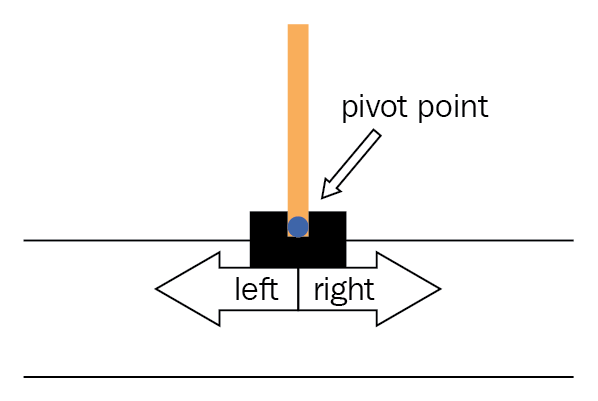
\includegraphics[width=.9\linewidth]{images/openai_gym.png}
  \caption{The OpenAI CartPole environment}
\end{figure}

\subsection{Training a Simple ANN agent}

First, we attempt to solve the problem with a simple MLP ANN agent that takes in
the four observations, and outputs as logits the probability of each action. The
action is then sampled from a 2-outcome categorical distribution with the logits
as the outcome probabilities. We do this so we can compare the performance of
the policies, learnt under the same conditions (learning rule, environment
parameters etc.).

Since SLAYER uses PyTorch, we implement vanilla policy gradients in PyTorch to
train the MLP agent. We use Sacred~\cite{klaus_greff-proc-scipy-2017} to log and
ensure reproducibility of our experiments.\footnote{This repository is hosted on
Github at \url{https://github.com/jethrokuan/snnrl/}. The repository is private,
request access as required.}

Experiments show that the ANN model learns to solve the environment quickly when
trained with VPG, as shown in \autoref{fig:vpg_mlp}. The agent obtains an
average episodic return of 200, ``solving'' the environment at 2000 time-steps.

\begin{figure}[htbp] \centering
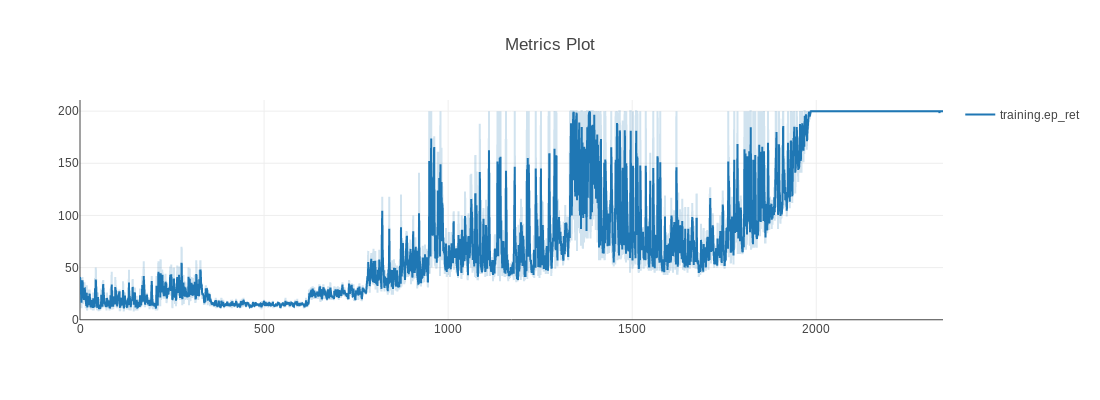
\includegraphics[width=.9\linewidth]{images/vpg_mlp.png}
\caption{\label{fig:vpg_mlp} Plot of average episode returns over time-steps for
a simple MLP agent.}
\end{figure}

\subsection{Training a SNN agent}

Similarly, we attempt to train the SLAYER model to solve the CartPole-v0. Each
SLAYER layer takes in a spike train as input and produces a spike train as
output. The objective function for supervised learning tasks such as
classification is defined in the paper, and is similar to
cross-entropy~\cite{NIPS2018_7415}.

Since the input to the Slayer model are spike trains, we require an encoder
mapping the environment observations into the fixed-length spike trains that
SLAYER accepts,as shown in \autoref{fig:slayer_rl}.

\begin{figure}[htbp] \centering
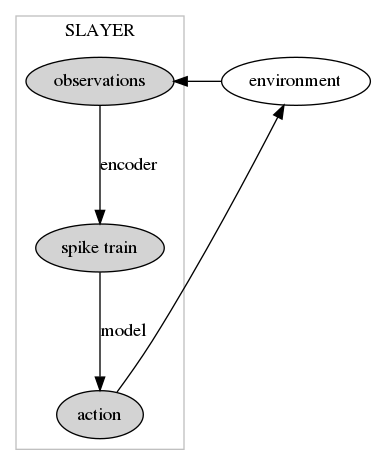
\includegraphics[height=7cm]{images/snn_encode.png}
\caption{\label{fig:slayer_rl} The SLAYER model requires an additional encoder
to transform the observations into spike trains as input.}
\end{figure}

We encode the observations by modelling the observations as Poisson
processes~\cite{heeger2000poisson}. First, we convert each of the four
observations into 2 non-negative observations: their absolute value, and their
sign. A negative value has an observation value of 0, and a positive value has
observation value of 1. We divide time into short, discrete intervals
\(\delta t\), and generate a sequence of random numbers \(x[i]\) uniformly
between 0 and 1. For each interval, if \(x[i] \le r \delta t\), generate a
spike. We produce spike trains of 300 time-steps as input to the SLAYER model
from the 8 observation values (scaled appropriately).

As shown in \autoref{fig:snn_vpg}, the SLAYER model fails to learn to solve the
problem.

\begin{figure}[htbp] \centering
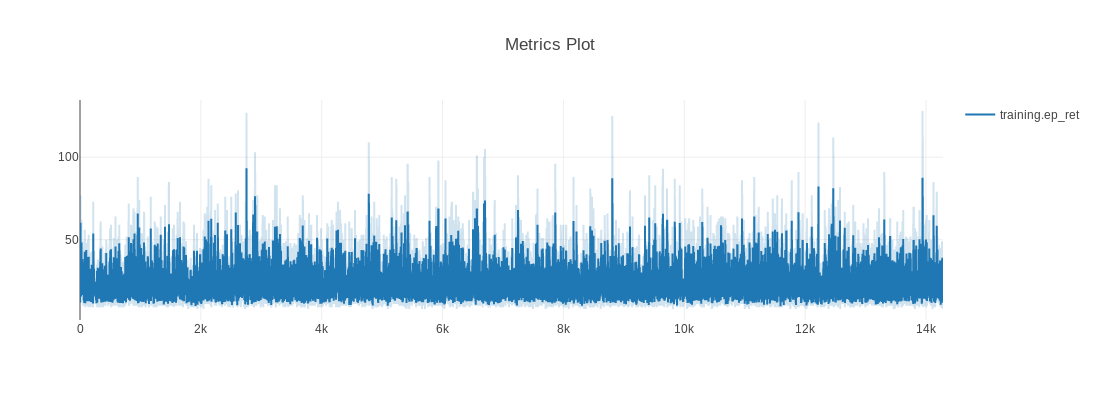
\includegraphics[width=.9\linewidth]{images/slayer_poisson.png}
\caption{\label{fig:snn_vpg} The SLAYER model with a Poisson encoder for the
observations fails to learn to solve the problem.}
\end{figure}

The problem likely resides in way encoding is done. The domain of the value of
some observations in the Cartpole environment is the range over all real
numbers, and encoding values over the entire range of real numbers is
tricky. There is no linear mapping, and changes in observation values may not
result in changes of noticeable magnitude in the mapped value.

There has, however, been works on encoding images into spike trains.  This is
particularly common as many spiking neural architectures are evaluated on a
converted MNIST image dataset. Hence, we move towards training spiking neural
networks on image observations.

\subsection{The ImageCartpole Environment}

To bypass the encoding issue described earlier, we turn towards training agents
on the pixels of the environment. We create a Cartpole environment such that the
observation is the difference in pixels of the current frame and the previous
frame. We term this modified environment ImageCartpole.

We train a simple CNN on this environment, using VPG.\@ Training this agent takes
significantly more time, as seen in \autoref{fig:imagecartpole_cnn}. However,
the agent is still able to learn from the observations, suggesting that this
environment is solvable by a SNN agent.

\begin{figure}[htbp] \centering
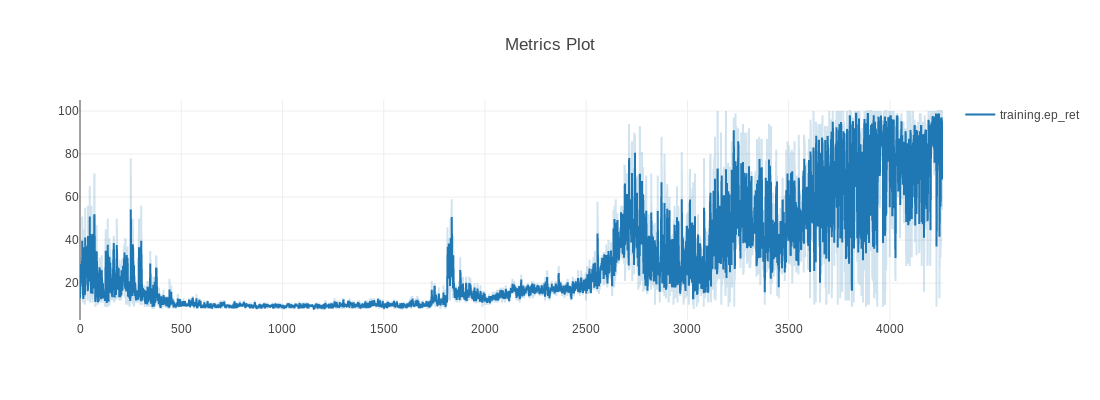
\includegraphics[width=.9\linewidth]{images/imagecartpole_cnn.png}
\caption{\label{fig:imagecartpole_cnn} Plot of the average episode return of a
CNN agent on the ImageCartpole environment over time.}
\end{figure}

At the time of submission, the SNN agent is unable to learn a good policy, but
more engineering work is required before any conclusions can be made.

\section{Future Work}

It is hoped that the SLAYER model is able to learn to solve simple environments
such as the Cartpole environment. Once it is established that gradient-based RL
methods also work for training SLAYER, we would move on towards milestones 3 and
4. If we are unable to learn a good policy via existing reinforcement learning
methods, some exploration into tweaking the learning rules or spiking neural
architecture is warranted.

As a closing thought, the way the cartpole environment is currently being used
also does not fully utilize the power of spiking neural networks. At each
time-step, observations are converted to full spike trains. SNNs are often able
to make predictions based on early spikes, albeit less reliable. This is not
exploited in the current environment formulation, where a full spike train of
fixed length is received before an action is taken.

In my idealized formulation of RL environment for SNNs, the following should be
satisfied:

\begin{enumerate}
  \item The action space should contain a no-op: in the case of the cartpole
  environment, this is as simple as adding the action of not applying force to
  the cart, instead of choosing between left or right
\item At each observation, the observation should be spikes, rather than spike
trains
\end{enumerate}

The SNN agent receives spikes at each time-step, and after gaining enough
confidence to take an action, it takes the action at that time-step. I
hypothesize that SNN agents should be able to solve such environments, by
exploiting the temporal information encoded in the relative timing between
spikes (in this case, number of timesteps) and that each spiking neuron stores
such temporal state, without the use of recurrent networks or replay buffers
common in current ANN setups.

\printbibliography

\appendix
\end{document}
